\RequirePackage{lineno} 
\documentclass[,superscriptaddress,showpacs,amssymb,amsmath,amsfonts,linenumbers,article]{revtex4-1}

\usepackage{graphicx}
\usepackage{dcolumn}
\newcolumntype{d}[1]{D{.}{.}{-1}} 
\usepackage{latexsym}
\usepackage{amsmath} 
\usepackage{url}
\usepackage{natbib}

\usepackage{mathtools}
\usepackage{framed}
\usepackage{diagbox}
\usepackage{multirow}
\usepackage{hyperref}
\usepackage{float}
\usepackage[margin=20mm]{geometry}
\usepackage{enumitem}

\newcolumntype{C}[1]{>{\centering\arraybackslash}m{#1}}

\pagenumbering{arabic}
\pdfminorversion=5 
\pdfcompresslevel=9
\pdfobjcompresslevel=9

\begin{document}

\begin{center}
\vspace{2cm}
{\LARGE Response to the Analysis WG Review (Round 1) of}\\[0.7cm] 

{\bf \large
 ``Quasi-free cross section measurements for the $\pi^{+}\pi^{-}$ electroproduction off the proton in deuterium with CLAS and a 2.039 GeV beam"\\[0.25cm]}

by Iu. A. Skorodumina, G.V. Fedotov, R.W. Gothe\\[1cm]
\end{center}


{\large Review Committee: Douglas MacGregor (chair), Nikolay Markov, James Ritman} \\[1.5cm] 

\vspace{0.25cm}
First we would like to thank the Review Committee for their comments and questions on the physics and also for the suggestions on improving the presentation of the results. The answers are listed below.

\vspace{0.75cm}
 
{\bf The review committee held a teleconference meeting on 10th October 2019 to discuss your analysis review paper. The review committee noted that your review addressed the detailed analysis of the data, but did not seek to offer a detailed physics interpretation of the results. The committee has some comments and questions on the paper, listed below, as well as some more minor suggestions to improve the typographic setting and the presentation. These are given in an annotated copy of the review file.}\\ \\


For the double-pion production off the bound nucleon both the experimental cross section extraction and its physical interpretation are very challenging tasks. It was decided to separate these two issues as the cross section interpretation can not be considered trustworthy without reliable establishing of the cross section itself. The analysis note is therefore devoted to the cross section extraction procedure, which along with the techniques established for the free proton case includes completely new methods related to the deuteron target case. The latter were elaborated during this study and therefore were set as the main focus of this analysis report.\\

Meanwhile, the physical interpretation of the results is underway and will be put into higher gear once the experimental part is approved. As briefly sketched in the Conclusion of the analysis report, it includes the comparison of the extracted cross sections with their free proton analogue (for both integral and differential distributions), detailed investigation of their difference and its dependence on the final state variables as well as some discussions on FSI and their manifestation in the double-pion channel. The details will be presented in the future journal publication on the subject. 

\vspace{0.5cm}

\begin{enumerate}[label=\textbf{\arabic*}.]

\item {\bf At line 108 you say that analysis review report presents integrated and single –differential cross sections. Are there any plans to extract and publish any other observables (e.g. doubly differential cross sections) from this data?}\\ \\
At the moment we do not have such plans. Presently we plan to concentrate on finalizing the physical interpretation of the extracted cross sections  and on the preparation of the journal publication, which will include both the details on the experimental cross section extraction and the physical interpretation of the obtained results. When this is complete, the extraction of other observables may be considered.


\item {\bf Around line 118 you say that the quasi-free data were taken under the same conditions as free proton data and this allows a comparison of the two data sets. It would be useful at this point to give an indication of the statistical accuracy obtained for the quasi-free study in comparison with the accuracy of the free proton study. Was there any normalisation of the quasi-free cross sections to the free proton cross-sections?}\\ \\
For the free proton integral cross sections for the majority of $(W,~Q^{2})$ points, the uncertainty $\delta_{\text{stat,~mod}}^{\text{tot}}$, which is the statistical uncertainty combined with the model dependence uncertainty, stays on a level of $\sim$~1\%-3\%. For the quasi-free integral cross sections for the majority of points this uncertainty is on a level of $\sim$~4\%-6\%. This information was added in the next to last paragraph of Introduction. No normalization of the quasi-free cross sections to the free proton cross-sections was performed. The detailed investigation of the difference between these two cross section sets will be a part of the physical interpretation of the result.

% The reasons for the latter to be higher are the following. First, the quasi-free cross sections have less statistics as only two reaction topologies are used against all four used in the free proton analysis. Then, in the quasi-free study the exclusivity cut is more strict than in the free proton analysis due to the need to remove FSI-background. Beside this, quasi-free cross sections have one extra source of the model dependence uncertainty related to the unfolding the effects of the target motion.

\item {\bf At line 135 you talk about using various targets for the hydrogen and deuterium runs. Was the same target cell used for both hydrogen and deuterium? You should say clearly what was the same and what was different.}\\ \\
The target cell was the same for the hydrogen and deuterium runs, but the target cell content was different. The clarification was added to the first paragraph of Chapter~2. 


\item {\bf At line 157 you say that you used the Monte Carlo generator TWOPEG-D. Did you try any other MC generators? And would they have given any different results for the detector efficiency? Is there any systematic uncertainty in the detector efficiency arising from the choice of generator used in the MC simulation?}\\ \\
We did not try any other MC generator, as TWOPEG-D is currently the only one existing EG that can properly simulate the effects of the initial proton motion for the process of the double-pion electroproduction.

In this study, the main issue that could impact the accuracy of the efficiency estimation was the inability of the free proton EG to reproduce the Fermi smearing of the missing quantities observed in the experimental distributions. As these distributions are subject to the exclusivity cut in order to select the reaction channel, this mismatch would cause inaccuracies in the estimated efficiency. Meanwhile, TWOPEG-D manages to reproduce this smearing, as illustrated by e.g. Fig. 2.31 from the analysis note, and therefore allows to avoid such inaccuracies.

One more issue that may influence the efficiency accuracy is the cross section shape approximation employed into an event generator. However, the degree of this influence depends on the size of bins in which the experimental cross section is extracted. For small bins, even the phase-space event generator manages to give adequate efficiency. Meanwhile, this analysis benefits from a fine binning in all kinematic variables and moreover, the cross section shape approximation used in TWOPEG-D is far more realistic than the phase-space approximation (see more details in Ref.~\cite{twopeg_d}). 

Taking into account all these arguments, we consider the efficiency estimated by TWOPEG-D to be trustworthy and would not expect any other EG to give a better result.


\item {\bf Around line 166, you state that the GSIM package does not properly reproduce the resolution of the drift chambers or the TOF system. You need to state clearly how bad the mismatch is and what its effect on the data analysis is. You immediately go on to say that the GSIM Post Processor is used to better match the resolution. You need to say how this works and whether or not it completely cures the problem. Is this a standard procedure? Has it been done in other analysis? Is there a suitable reference?}\\ \\
This analysis employs standard and well-established CLAS software for the purpose of simulating the detector response, which includes GSIM (GEANT SIMulation), GPP (GSIM Post Processor), and recsis (reconstruction software). This multi-stage simulation/reconstruction procedure is used in all CLAS data analyses as confirmed by e.g. Refs.~\cite{Markov:2014, Arjun, Ye_Tian:2017}.

As the resolution depends on kinematics and hence on experimental conditions, the GPP parameters intended to adjust the resolution (DC and TOF smearing factors) are typically determined individually for a particular dataset. This analysis uses the GPP parameters that were determined for the study described in Ref.~\cite{fedotov_prc}, which reports the measurements of the same reaction performed under the same experimental conditions (but off the free proton).

One can judge the quality of the employed GPP parameters for example by examination of missing quantities (such as missing masses), comparing their simulated distributions with experimental ones. The achieved match between them indicates properly chosen GPP parameters. In this analysis, a very good agreement between experimental and simulated missing quantities is observed, as confirmed by e.g. Fig. 2.31 from the analysis note. From this, one can conclude that the applied procedure completely cures the problem and does not seem to affect the analysis.

The related part of the text on page~8 was rewritten with the corresponding clarifications added.


\item {\bf Lines 179 to 187 are written using jargon in the style of an expert manual. Their meaning is not immediately clear.  It would be better to rewrite this section, providing more explanation of what was done, why it was done and what effect it has.} \\ \\
All events collected with CLAS are stored in a specific format, which is BOS format. This format is unique for CLAS and incorporates numerous BOS banks (e.g. HEVT, EVNT, DCPB, etc.), each containing a piece of specific information about a particular event. Each bank contains the set of variables, and their specific names and descriptions (e.g. $stat$, $gpart$, $DCstat$, etc.), indeed looking as jargon, are nevertheless well-established. The complete list of BOS banks (with all variables and their descriptions) can be found in Ref.~\cite{BOS}.

These lines describe an initial part of the event selection (some kind of event preselection), which is standard and performed in each CLAS data analysis. 

This part of the text was rewritten with more explanations added (pages~8-9).


\item {\bf In figure 2.1 is there an explanation for the downwards tail at $P_{e’}$ $\sim$1.8 GeV, seen in all six sectors? If there is, it would be useful to comment on it. We note that this effect is not seen in the simulations shown in figure 2.2. Is there any upper limit applied to the $P_{e’}$ data shown in Figure 2.1?}\\ \\
The region of the event excess below the main structure (including the mentioned tail) is attributed to the pion contamination, which is supposed to be partially rid of by the sampling fraction cut and will be further eliminated after the cuts in the CC. 

The events at $P_{e} \sim 1.8$~GeV came from the elastic scattering. The relative contribution from the pion contamination is about the same for all $P_{e}$, but since at our beam energy the event sample is dominated by elastic events, a pronounced tail from pions appears in this region. This effect is seen in FIG.~1 (here) plotted without log scale.

Beside this, the pion contamination in Fig.~2.1 looks so pronounced as the figure is plotted before all other cuts. A large part of the tail comes from the first CC segment, which turns out to be totally dominated by the pion contamination. This segment is later removed from the analysis by the fiducial cut in the CC plane given by Eq.~(2.1.10). This effect is illustrated by FIG.~1 (here), where the tail decreases significantly after the manual removal of the 1st CC segment. The pion contamination at other values of $P_{e}$ decreases as well.


\begin{figure}[htp]
\begin{center}
\framebox{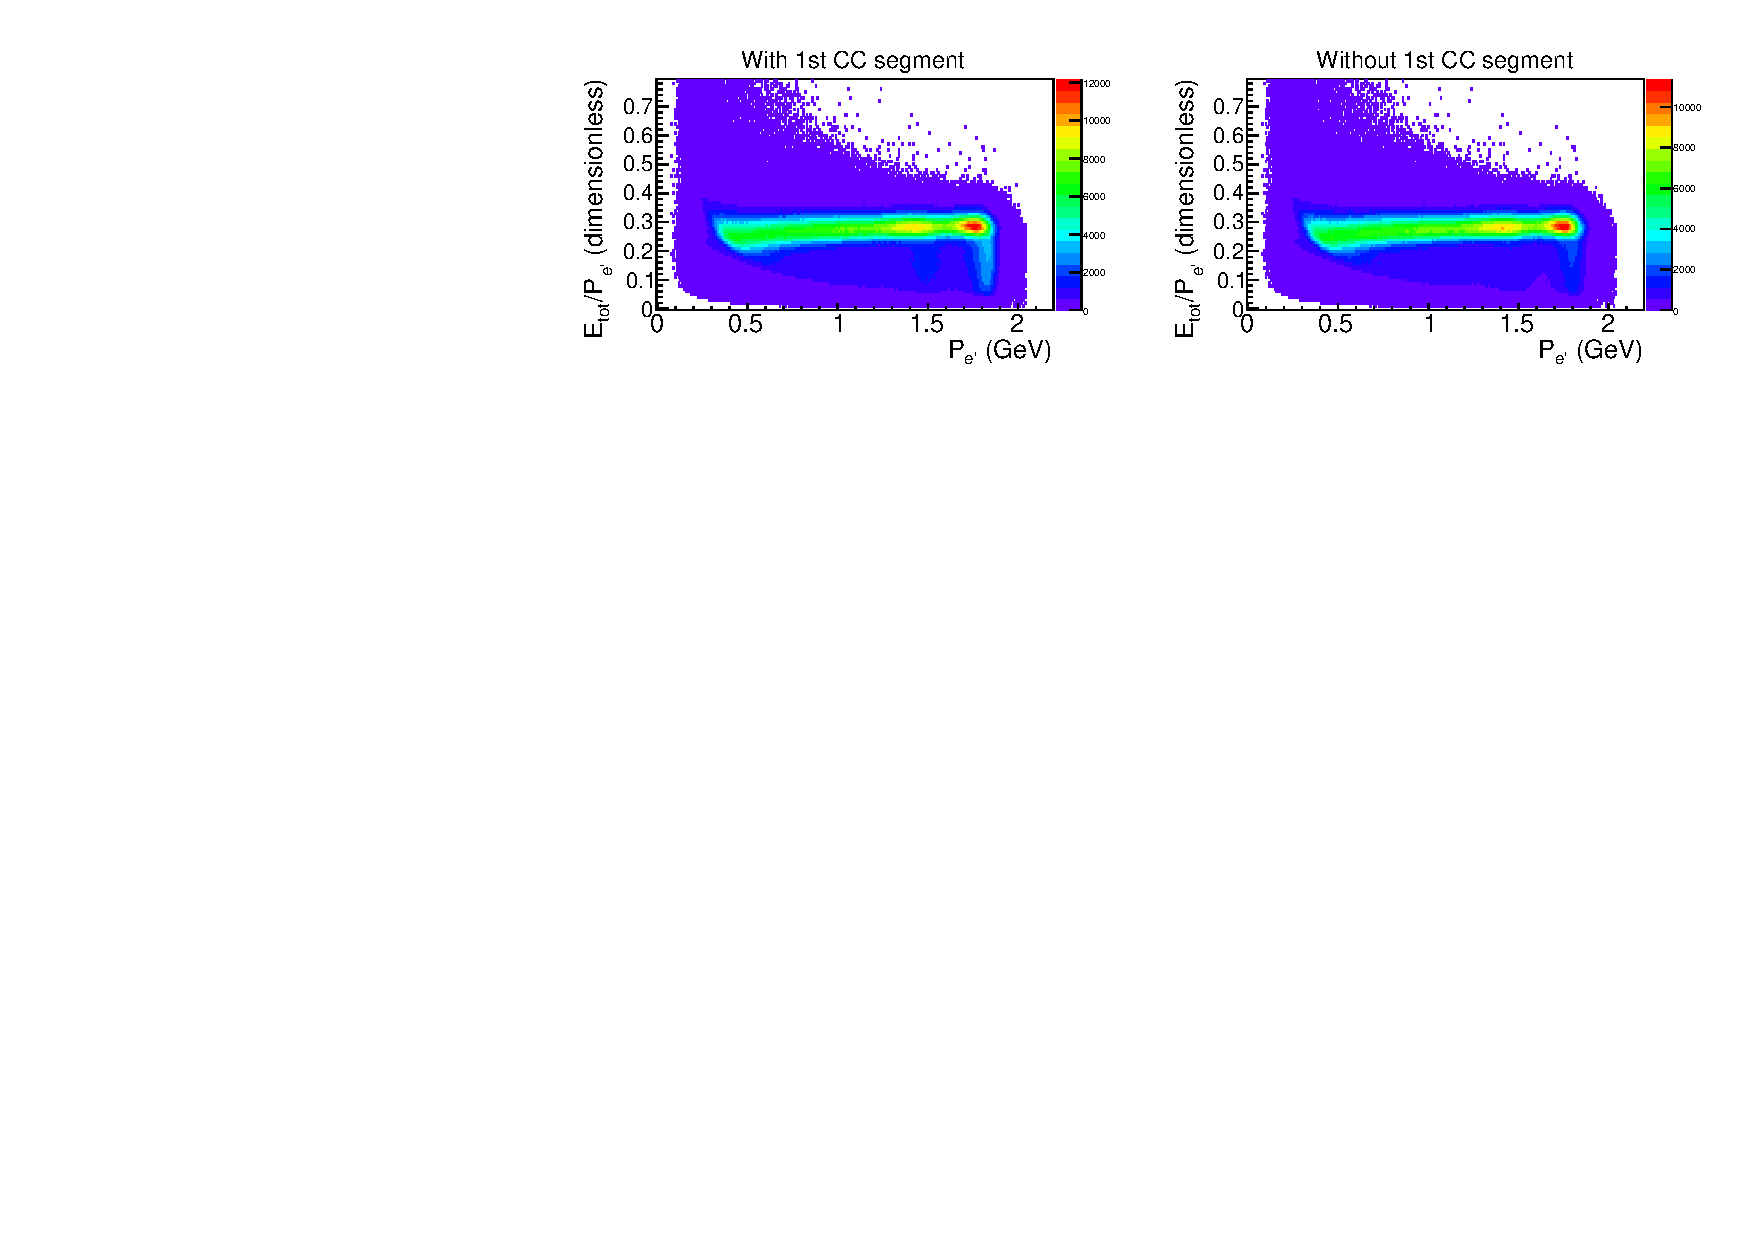
\includegraphics[width=10cm]{pictures/ectot2.pdf}}
\caption{\small  Examples of experimental sampling fraction distributions for Sector~1 and a small portion of analyzed statistics. Left: including the 1st CC segment. Right: excluding the 1st CC segment.} \label{fig:cc_plane_def}
\end{center}
\end{figure}


Note also that Fig.~2.1 is plotted for inclusive electrons, while Fig.~2.2 contains only double-pion events as only this exclusive channel was simulated. At the beam energy of 2.039~GeV the energy of the scattered electron for the double-pion production does not exceed $\sim$1.5~GeV as illustrated by Fig.2.2.

No upper cut on $P_{e’}$ is applied. It looks like the experimental distributions end at the beam energy value. 


\item {\bf In figure 2.4 it might be clearer to show the difference between $\theta_{CC}$ and the average (or expected) value for each segment. $\Delta \theta_{cc}$ would then be centred around zero. This would give a better presentation and show clearly whether the applied cuts were consistent across all the segments, which is difficult to judge from the given plots. As shown this figure is slightly on the small side.}\\ \\
FIG.~2 (here) shows the distribution of the quantity $\theta_{CC} - \theta_{CC}^{mean}$ versus segment for Sector 1, where $\theta_{CC}^{mean}$ is the mean value of the Gaussian function used for fitting the distribution of $\theta_{CC}$ for each segment. Black horizontal lines correspond to the $\pm$ 4$\sigma$ cut applied to eliminate background noise and accidentals. It looks like the $\theta$ distributions are getting wider for larger segment numbers and the applied cut follows this widening. As this cut is an auxiliary one, it was made rather loose in order to avoid unnecessary loss of good electrons.

\begin{figure}[htp]
\begin{center}
\framebox{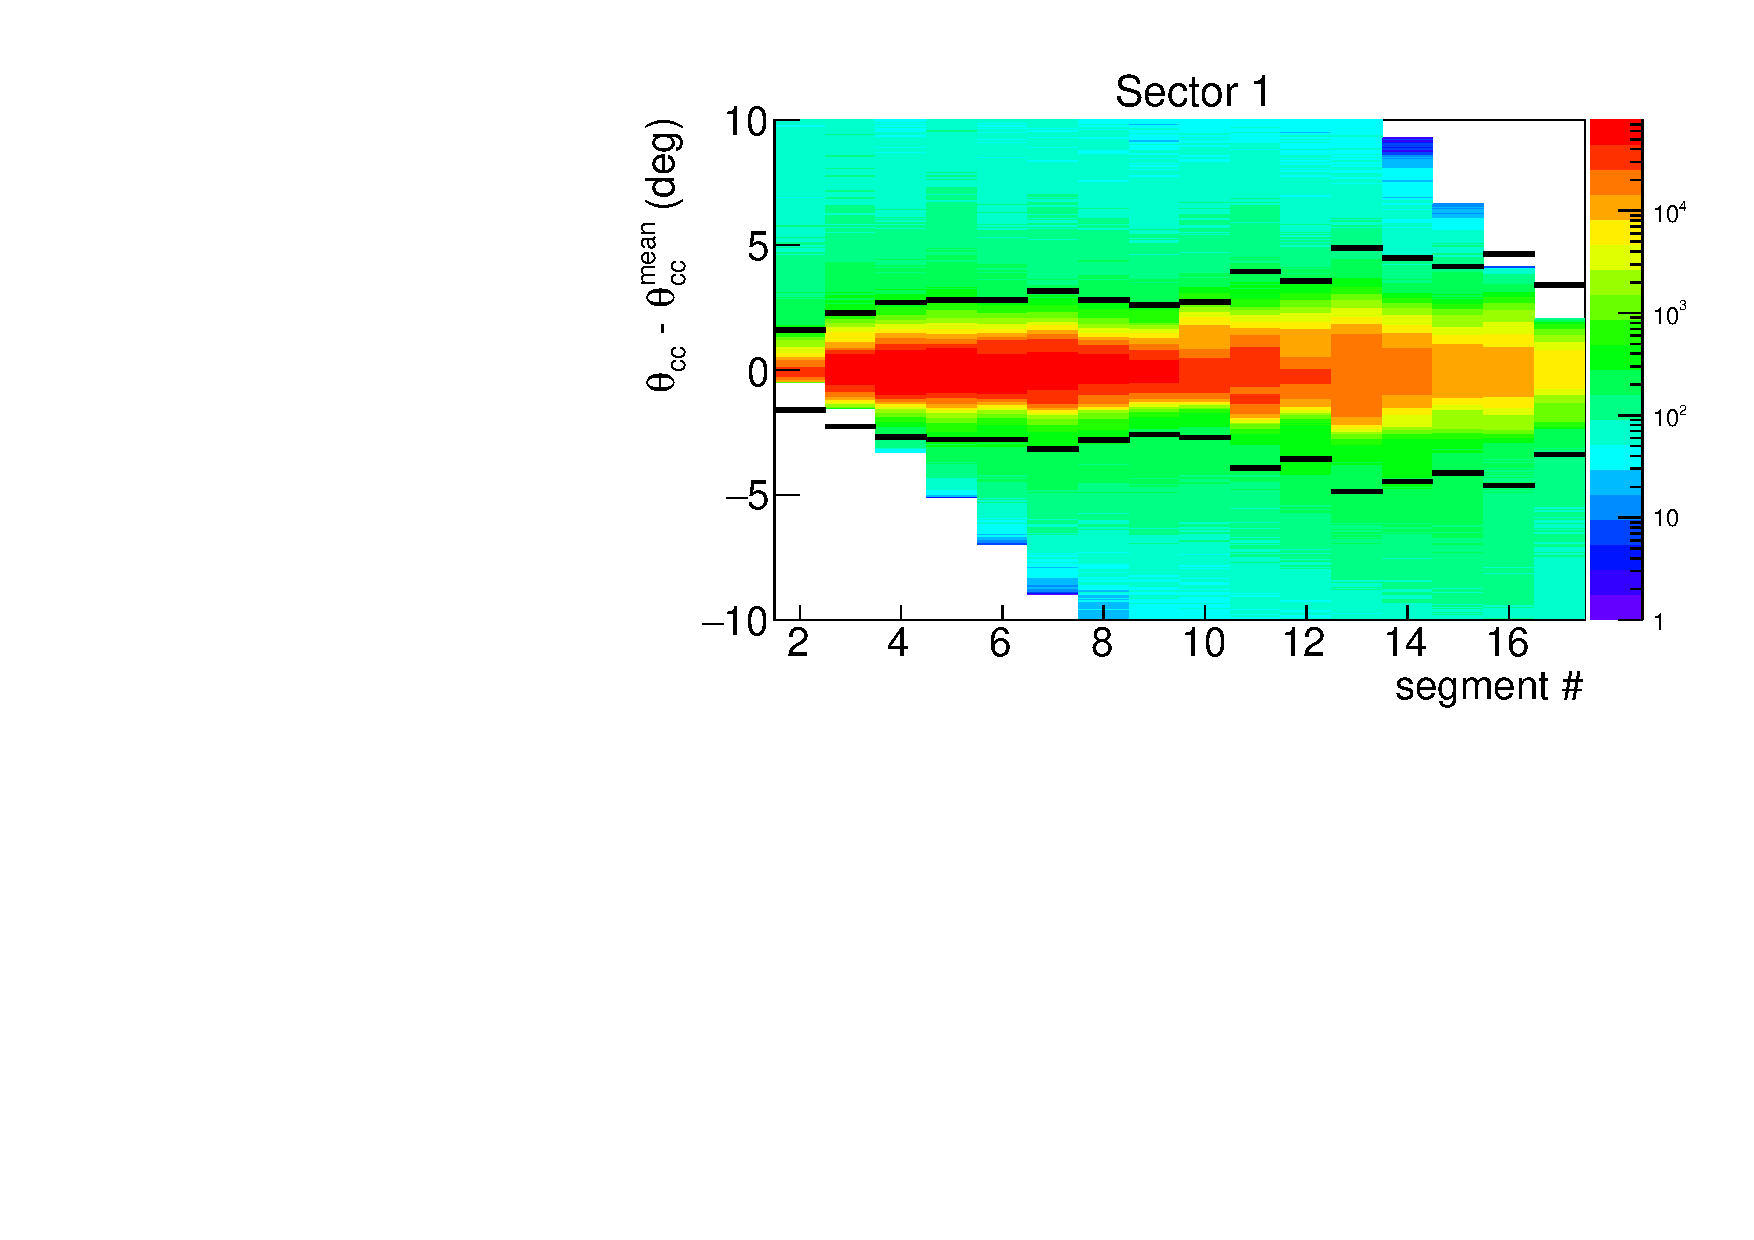
\includegraphics[width=7cm]{pictures/thvsseg.pdf}}
\caption{\small Distribution of the quantity $\theta_{CC} - \theta_{CC}^{mean}$ versus segment for Sector 1, where $\theta_{CC}^{mean}$ is the mean value of the Gaussian function used for fitting the distribution of $\theta_{CC}$ for each segment. Black horizontal lines correspond to the $\pm$ 4 $\sigma$ cut applied to eliminate background noise and accidentals.}  \label{fig:cc_plane_def}
\end{center}
\end{figure}

For this cut, we prefer the way of presentation offered in the analysis note as it seems to be more natural and advantages clear visual perception of (i) the whole available range of $\theta_{CC}$ and (ii) the undisturbed distribution of background noise that is subject to removal by this cut.

\item {\bf In figure 2.5, how much data is removed by applying the green cut, which appears to have the largest effect? Have any MC simulations been carried out to show whether these cuts introduce any bias into the shape of the final differential cross sections?}\\ \\
The cuts that correspond to the red and blue curves in Fig.~2.5 are not expected to affect the cross sections as they do not impact the main part of the photoelectron spectrum (which corresponds to good electrons further used in the analysis) and influence only the noise-peak part. 

The cut that corresponds to the green curve in Fig.~2.5 is just a geometrical cut analogous to fiducial cuts and therefore should have a similar effect on the cross sections. This issue was checked during the analysis with the conclusion that the variation of the cut value from 0.5 to 0.8 does not exert any significant influence on the extracted cross sections.

The cut that corresponds to the green curve in Fig.~2.5 removes 12\%, 19\%, 9\%, 15\%, 8\%, and 12\% of events for the Sectors from 1 to 6, respectively (compared to the distributions shown in blue).


\item {\bf In section 2.1.2 has any energy loss correction been applied in calculating beta for protons?}\\ \\
The energy loss correction to the proton momentum is applied before the $\beta$ versus momentum cut. When establishing the cut, the $\beta$ versus momentum distributions were filled using the corrected momentum.

\item {\bf In line 396 there seems to be an issue with paddles \#48 in all of the sectors. Is there some reason for this?}\\ \\
%According to Ref.~\cite{clas_tof_paddles}, each sector of the CLAS TOF had 57 scintillators arranged in four panels. However, ``in order to reduce the number of electronics channels, some of the scintillators have been ganged together electronically. Since there is no way to tell which of the two scintillators were struck by looking solely at TDC and ADC data, these counters are treated as single double width unit." In the panel 3 the TOF paddles \#40, \#41, and \#42 are the ganged scintillators \#40-\#41, \#42-\#43, and \#44-\#45, respectively. In panel 4, all remaining scintillators are ganged together in pairs to form paddles from \#43 to \#48.
%Most of the paddles with number $\geq$40 have the problem of double-bands in the $\beta$ vs $p$ distributions, which seems to originate from the fact that the timing information from the paired scintillators was not synchronized. 
Signals from paddles \#48 turned out to be completely unreliable as they contain enormous amount of events. This can be explained by the assumption that outputs from several scintillators were assigned to these paddles. This assumption is confirmed by FIG.~3 (here), which shows an example of particle coordinates distributions in the SC plane (for protons) and illustrates the problem with paddle \#48.


\begin{figure}[htp]
\begin{center}
\framebox{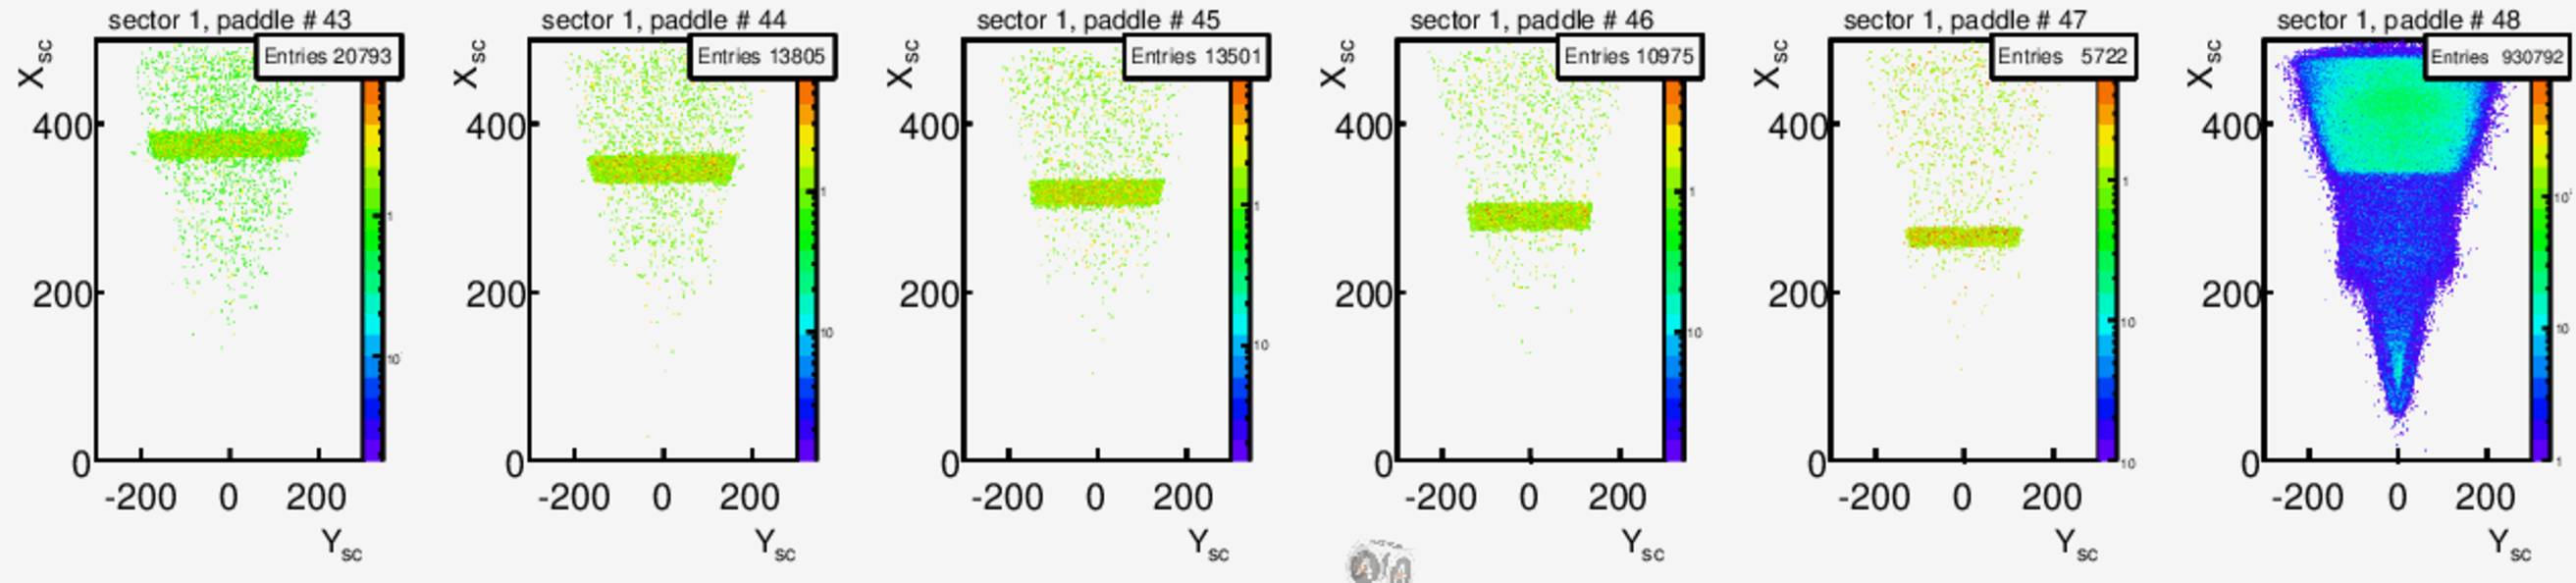
\includegraphics[width=0.95\textwidth]{pictures/paddles.pdf}}
\caption{\small Distributions of the particle coordinates (for protons) in the SC plane for Sector 1 and paddles from \#43 to \#48.}  \label{fig:cc_plane_def}
\end{center}
\end{figure}


The problem is present in all sectors. The corresponding paddles therefore were removed from the analysis.

This issue with paddles \#48 is also observed in other studies related to ``e1e" run period (see e.g. Refs.~\cite{fedotov_prc,Ye_Tian:2017}).


\item {\bf In figure 2.8 the 3rd and 4th columns should be interchanged, so the corrected data is presented in the same order as the uncorrected data. Are the problems with problematic paddles checked once in the analysis or on a run-buy-run basis?}\\ \\
The plots in Figs.~2.8 and 2.9 are arranged in a different way, and now they seem to look better. 

The problematic paddles were checked with the total analyzed statistics. It does not seem that run-by-run analysis would provide enough statistics to judge a paddle quality.

\item {\bf In figure 2.9 there appears to be more than one correction applied. How is this done? Is it on an event-by-event basis? Or is some other way? This needs a comment. Could a third correction be needed. There seems to be some residual double structure in the corrected spectrum for Paddle 46 in Sector3. Again the 3rd and 4th columns should be interchanged.}\\ \\
The plots in Figs.~2.8 and 2.9 are arranged in a different way, and now they seem to look better. 

For double-band paddles the correction was done in the following way. First, the positions of each band were identified by Gaussian fitting. Then, the midpoint between the bands was found. Then, events above this midpoint were shifted with the upper band position, while events below the midpoint were shifted with the lower band position. The correction is done in an event-by-event basis.

Some double-band paddles indeed had some additional low-intensity structures. The most pronounced of them were treated as a very weak third band and shifted to the zero position using the procedure described above. Others were ignored, as the overall impact of the timing correction on the cross section is marginal.

\item {\bf In figure 2.10 there is evidence of additional bands of particles. Do you know what these are?} \\ \\
FIGURE.~4 (here) shows the $\beta$ versus momentum distributions for positive hadron candidates with the superimposed black curves for the nominal $\beta$ calculated under exact hadron mass assumptions (see Eq.~(2.1.16) in the analysis note). The mass of the following hadrons was assumed: in the upper plot -- muon, pion, and kaon, while in the lower plot -- kaon, proton, and deuteron. As seen from the plots, the black curves match perfectly the corresponding experimental bands, so these bands can be attributed to the considered hadron types.

\begin{figure}[!ht]
\begin{center}
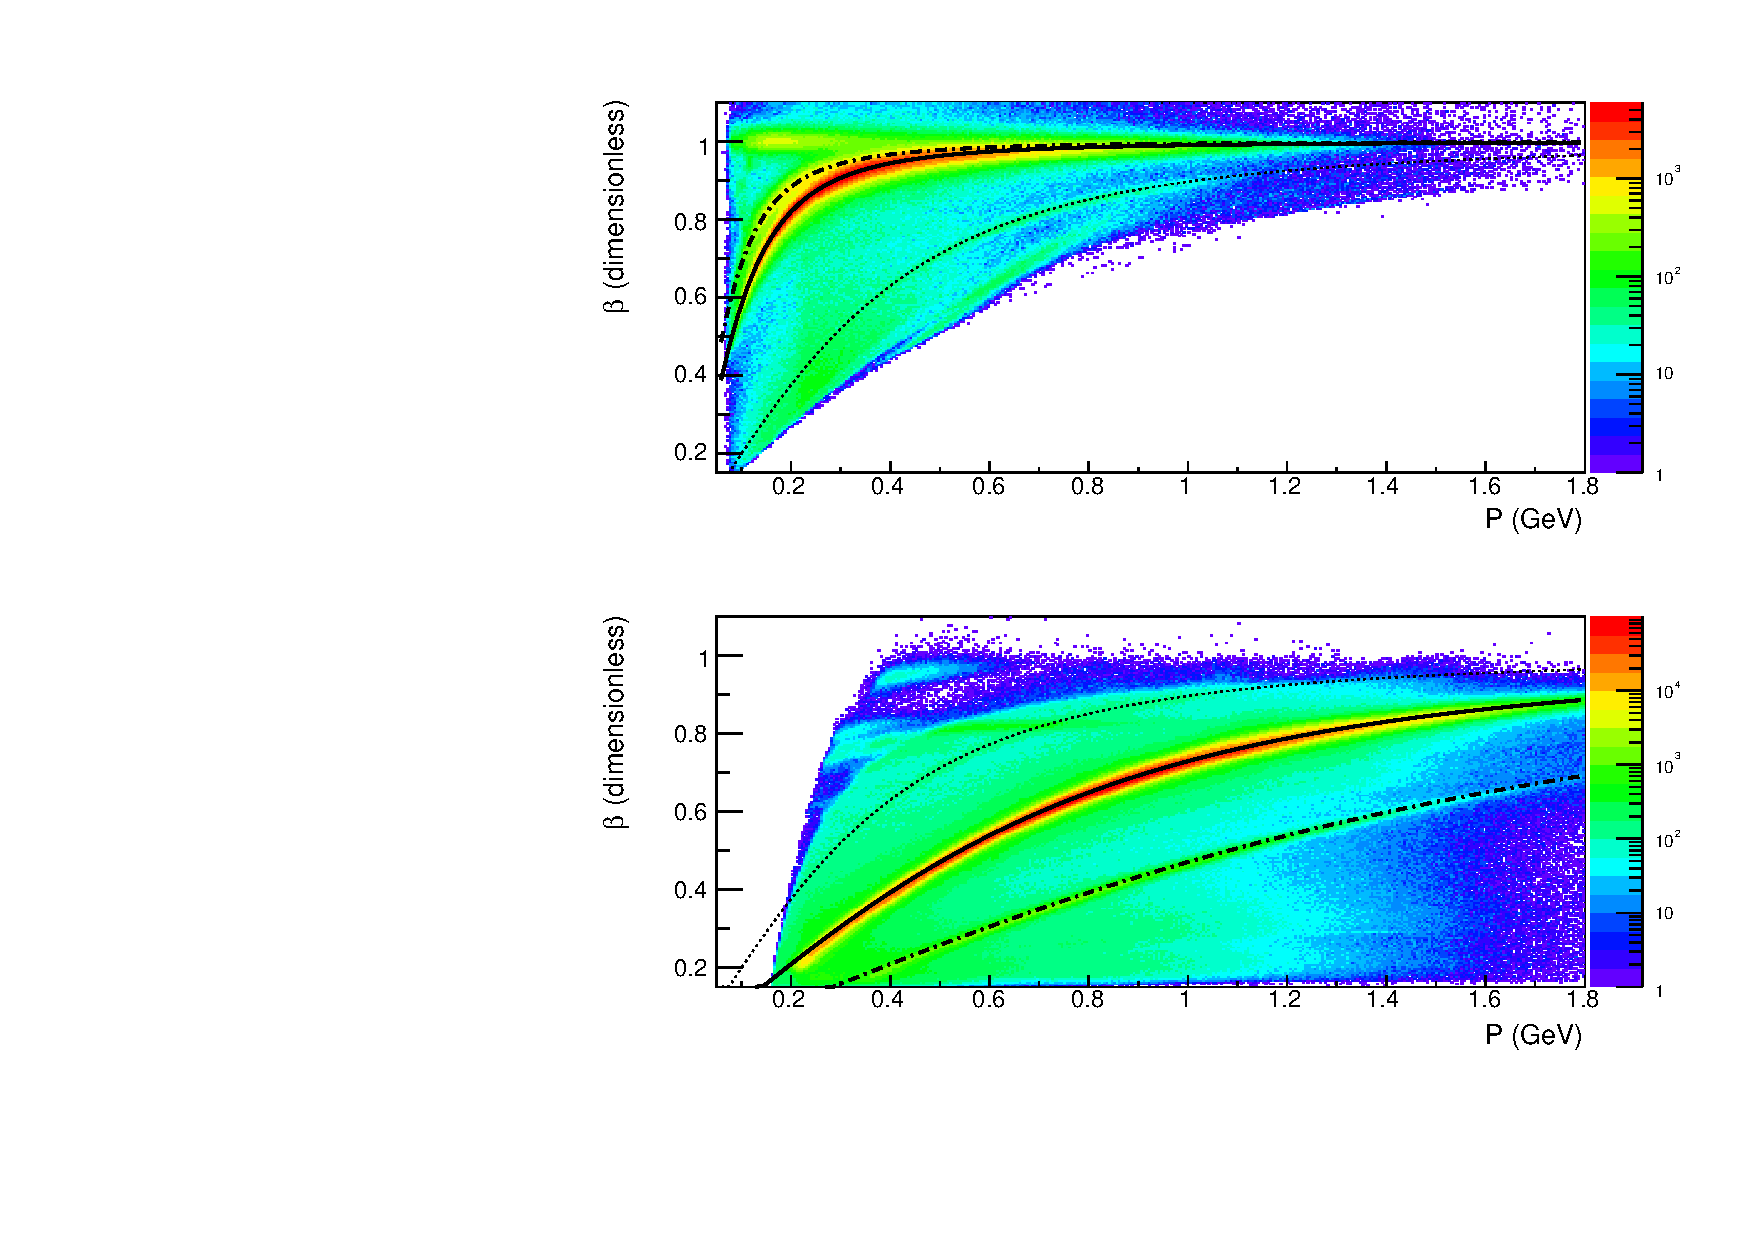
\includegraphics[width=10.5cm]{pictures/hadr_id.pdf}
\end{center}
\caption{\small $\beta$ versus momentum distributions for positive hadron candidates. Black curves correspond to the nominal $\beta$, which is calculated under the exact mass assumption for a particular hadron type. Upper plot: the solid curve is for the pion mass assumption and the dot-dashed curve is for the muon mass assumption. Lower plot: the solid curve is for the proton mass assumption and the  dot-dashed curve is for the deuteron mass assumption. The thin dotted line in both plots is for the kaon mass assumption. }  
\end{figure}
\begin{figure}[!ht]
\begin{center}
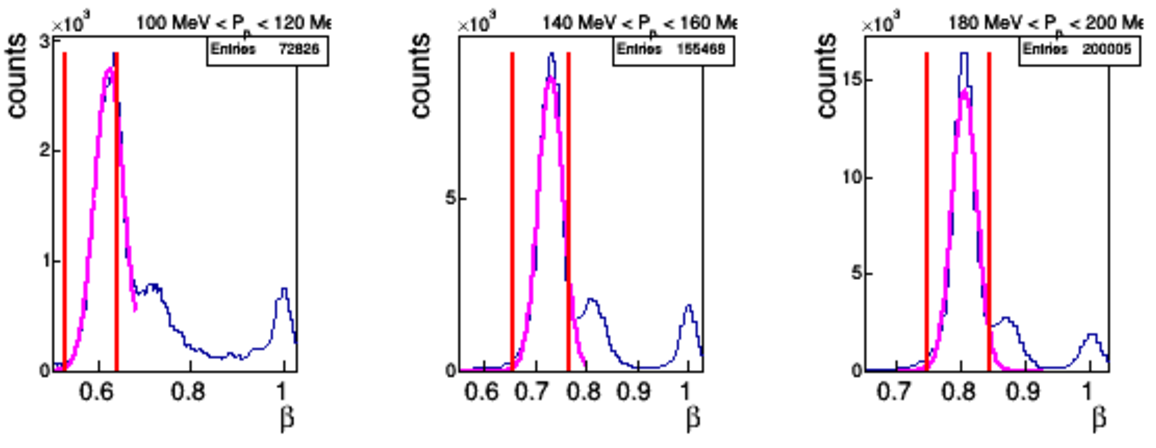
\includegraphics[width=10.5cm]{pictures/pip_id1.pdf}
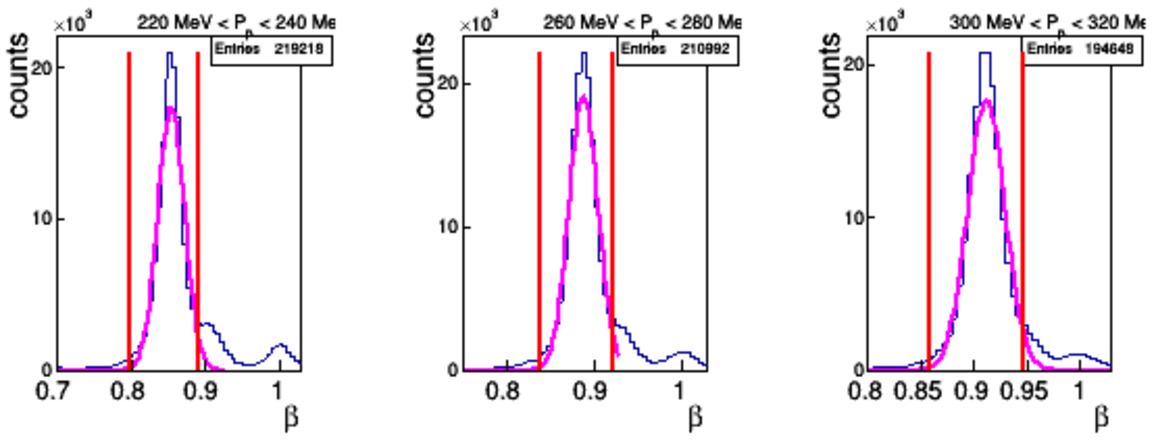
\includegraphics[width=10.5cm]{pictures/pip_id2.pdf}
\end{center}
\caption{\small 1D slices of the 2D $\beta$ vs momentum histogram for positive pion candidates in the low-momentum region, i.e. from 0.1~GeV to 0.32~GeV that corresponds to the first six black point-pairs in Fig.~(2.10) in the analysis note. The purple curves show the Gaussian fits of the main pion peak. The red lines mark the positions of points which will be further subject to fitting by the function (2.1.19) to determine the upper and lower cut boundaries. The left red line is at the position of $mean-3\sigma$, while the right line is at the position of $mean+a\sigma$, where $a$ = 0.5, 1.5, 2, 2, 2, 2 for the slices from one to six, respectively. }  
\end{figure}

Note that in FIG.~4 pion and proton candidates are shown in separate plots as they we subject to the preselection to simplify the analysis process.

\item {\bf In the case of the cuts on positive pions, there is an intense region (yellow) just outside the cut at low $P_{\pi^{+}}$ (0.15-0.28 GeV), while all the other cuts include all of the yellow region. You could be losing some $\pi^{+}$ here. Is this just one or two paddles? Can we see an example of a slice showing the $\pm 3 \sigma$ cut used to determine equation 2.1.19, to check that it is Gaussian in nature?}\\ \\
The pion band has a neighboring less intensive upper band, which is attributed to muons as the curve with the exact muon mass assumption perfectly matches this band (see FIG.~4 here and the answer to the previous question). The two bands are poorly separated as masses of the pion and muon are very close to each other. However, in the low momentum region, they can be visibly distinguished.

More details can be seen in FIG.~5 (here), which shows 1D slices of the 2D $\beta$ vs momentum histogram for the low-momentum region, i.e. from 0.1~GeV to 0.32~GeV that corresponds to the first six black point-pairs in Fig.~2.10 in the analysis note. As seen, three separate peaks can be distinguished, which are attributed to pions, muons, and positrons (at $\beta = 1$) from left to right.

To separate the pion peak the following procedure was used. The main pion peak was fit by Gaussian functions shown in purple in FIG.~5. Then the positions of the left and right points were determined, which will be further subject to fitting by the function (2.1.19) to obtain the lower and upper cut boundaries, respectively. The red lines in FIG.~5 mark these positions. The left red line is always at the position of $mean-3\sigma$, while the right line is at the position of $mean+a\sigma$, where $a$ = 0.5, 1.5, 2, 2, 2, 2 for the slices from one to six, respectively. For the points from seven to eleven, $a = $~2.5, and for all other points to the right $a = $~3 as usual.

This procedure allows narrowing a bit the upper boundary of the pion id cut in the low momentum region, getting rid in this way from the undesired muon band (and actually from the positron band, too). The amount of pions lost in this way is not expected to be significant, but the selected event sample refines, which allows lower background in the missing mass distributions in the next analysis steps. The latter, meanwhile, is very important for this analysis, because the channel selection by the exclusivity cut is already complicated by Fermi smearing and FSI. 

\item{\bf  In footnote 6 is is said that the $\pm$3 sigma cut was not applied below $P_{\pi}$ = 0.54 GeV. What exactly was done here? This is not clear. Could this be part of the issue? It is suggested that there is also a separate muon band, but this is not obvious from the figure.}\\ \\
See FIGS.4~and~5 (here) and the answers to the two previous questions.

\item {\bf In cuts 2.3.3 and shown in figure 2.18, the proton $\theta^{max}$ cut is much tighter than the corresponding pion cut. Based on the intensity distributions a cut of around 80 degrees (rather than 60 degrees) would seem to be comparable to effect of the pion cut. Can you say why the proton cut is so tight?} \\ \\
The proton $\theta^{max}$ cut was set at 60 degrees on purpose. It turned out that the portion of protons, which have undergone FSI, rises dramatically with increasing $\theta$. Specifically, for $\theta > $ 60 degrees, quasi-free protons vanish and only FSI-disturbed protons are left. 
For pions, this correlation, although being observed as well, is not as strong as for protons. This was found out when comparing experimental missing momentum distributions with simulated ones (as in Fig.~2.29 in the analysis note) in different slices of final hadron angles. 

This observation is in agreement with the fact that large-angle protons have low momenta and hence are more likely to interact in the final state (as the interactions probability is thought to be higher for slower hadrons). 

The analogous distributions from the free proton analysis are less populated with events in the region of $\theta \geq$ 50 than the distributions of this analysis. Beside this, the simulation (that does not include FSI) also does not show many events in this region.

Taking into account these arguments, we concluded that setting $\theta^{max}$ to 60 degrees would not cause any loss of good quasi-free protons but may help to minimize FSI contamination, hence clearing up the missing mass distributions and facilitating the exclusivity cut.

\item {\bf In figure 2.20, sector 5 data, there appear to be some additional inefficient bands which have not been cut out. Is there a reason for this?}\\ \\
These small inefficiencies are thought to originate from dead DC wires. They were not cut out because they were considered as minor. The $\theta$ versus momentum cuts are established as a compromise between the intention to cut out as many inefficiencies as possible and the desire to keep enough statistics and (which is more important) to maintain adequate coverage of the reaction phase-space. Removing too many zones from the reaction phase-space causes an unnecessary rise in the empty cell amount, hence increasing the model dependence of the cross sections.

\item {\bf In figure 2.21 can you say how much of the data has been cut out by the cuts applied?}\\ \\
The total Faraday Cup charge without the quality check cuts is 4167.79 $\mu C$, and after the cuts, it is 3675.52 $\mu C$. Therefore, around 12\% of statistics has been cut out by these cuts.

\item {\bf In line 626 you say the entrance and exit windows were 15m thick?}\\ \\
``15-m-thick" was changed to ``15-$\mu$m-thick".

\item {\bf Lines 720-724: Can you quantify how much additional data is obtained by using the exclusive topology. At present it only says it gives a slight increase in statistics, which is not a precise description. You also say that the exclusive topology reduces the number of empty cells. Can you say how many additional cells are populated by this topology, which were not filled by the $\pi^{-}$ topology?}\\ \\
The contribution of the fully exclusive topology to the total analyzed statistics varies from $\sim$5\% near the reaction threshold to $\sim$25\% at $W \sim$ 1.7 - 1.8~GeV.

The contribution of the fully exclusive topology to the total amount of analyzed non-empty cells grows from $\sim$1\% near the threshold to $\sim$10\% at $W\sim$~1.5~GeV and stays on this level up to $W\sim1.8$~GeV. Note that binning is $W$-dependent and the total considered number of bins grows from $W = 1.3$~GeV to $W = 1.475$~GeV and then is kept the same for higher $W$ (see Tab.~3.1 in Sect.~3.4 of the analysis note).

\item {\bf Line 734: You state that the momentum of the proton in the initial state can be deduced by momentum balance in the exclusive topology. What is the resolution of this missing momentum reconstruction?} \\ \\
The resolutions of such momentum reconstruction would be determined mostly by the detector resolution (being also affected by other factors such as radiative effects and FSI).

One can estimate this resolution from the simulation. FIGURE~6 (here) shows the distributions of the momentum difference $P_{gen} - P_{X}$, where $P_{gen}$ is the Fermi momentum for a particular generated event, while $P_{X}$ is the missing momentum for the corresponding reconstructed event. The missing momentum $P_{X}$ is calculated according to Eq.~(2.4.1) in the analysis note. Each plot corresponds to a particular 100-MeV-wide bin in $W$.  All distributions are normalized to their maxima and fit by Gaussians. The $\sigma$ value of the fit is provided in each plot to facilitate the resolution judgment.

\begin{figure}[!ht]
\begin{center}
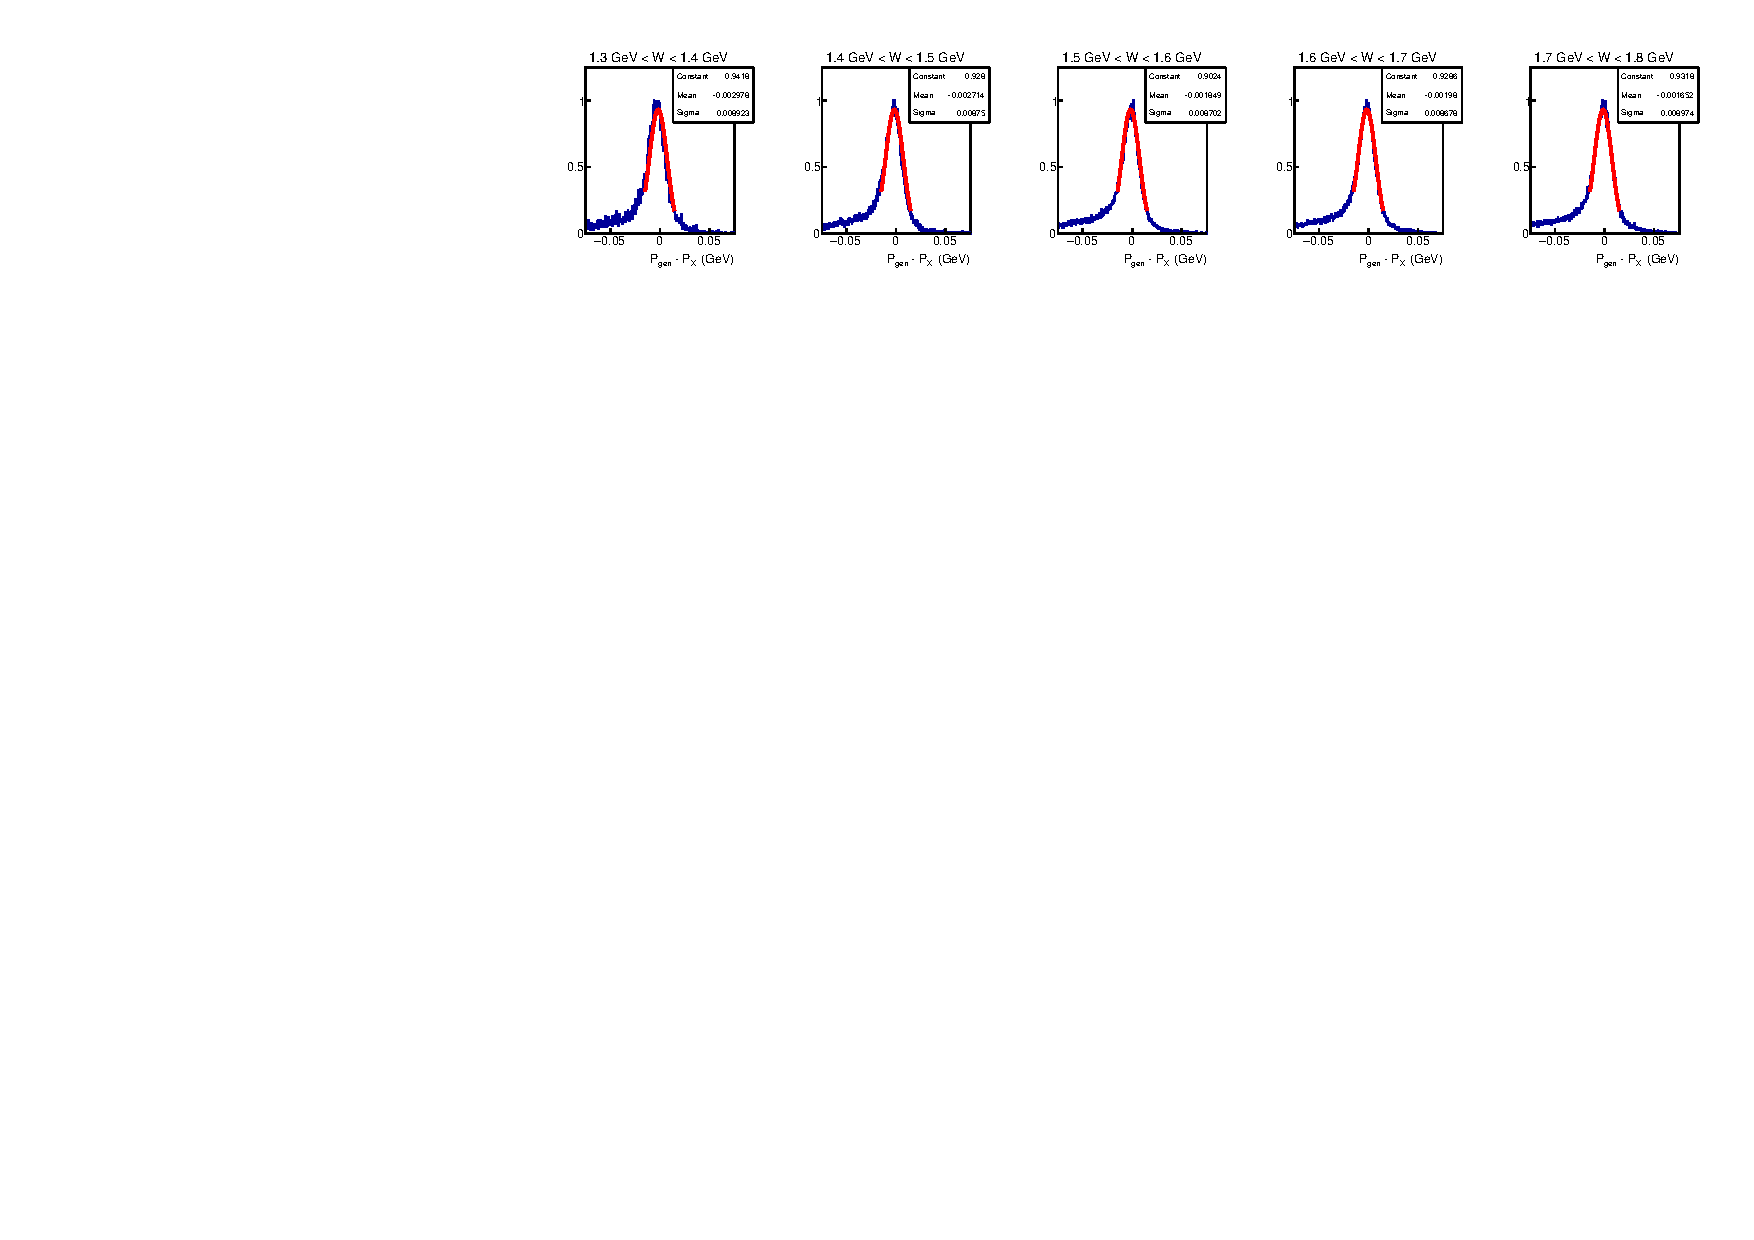
\includegraphics[width=\textwidth]{pictures/fermi_mom_res2.pdf}
\end{center}
\caption{\small Distributions of the momentum difference $P_{gen} - P_{X}$, where $P_{gen}$ is the Fermi momentum for a particular generated event, while $P_{X}$ is the missing momentum for the corresponding reconstructed event. The missing momentum $P_{X}$ is calculated according to Eq.~(2.4.1) in the analysis note. Each plot corresponds to a particular 100-MeV-wide bin in $W$. All distributions are normalized to their maxima and fit by Gaussians. }  
\end{figure}

Note that in this analysis the missing momentum $P_{X}$ is used only for the missing momentum cut applied for the removal of the FSI-disturbed events (as described in Sect.~(2.4.1) of the note).


\item {\bf Lines768 and 769 are rather clumsily written and need to be rephrased.}\\ \\
The whole paragraph was rewritten (pages~47-48).

\item {\bf In figure 2.30 the difference between the blue and black lines to the right of the peak is attributed to a three pion background. This is described as a peak at $m_{\pi}^{2}$, but hardly appears to be peak-like. Could this background be simulated in the MC?}\\ \\
The three-pion background manifests itself as a peak at $m_{\pi}^{2}$ in the distributions of the quantity $M_{X[0]}^{2}$. For the reaction off the free proton this peak, being smeared by the detector resolution and radiative effects, is seen as widened and flattened structure (but still peak-like) well-separated from the main distribution. This can be seen in FIG.~7 (here), which is taken from Ref.~\cite{fedotov_prc}. This figure shows the distributions of the quantity $M_{X[0]}^{2}$ for the double-pion electroproduction off the free proton in two 25-MeV-wide bins in $W$. Three-pion background is seen as a structure at the right side of the main peak.

\begin{figure}[!ht]
\begin{center}
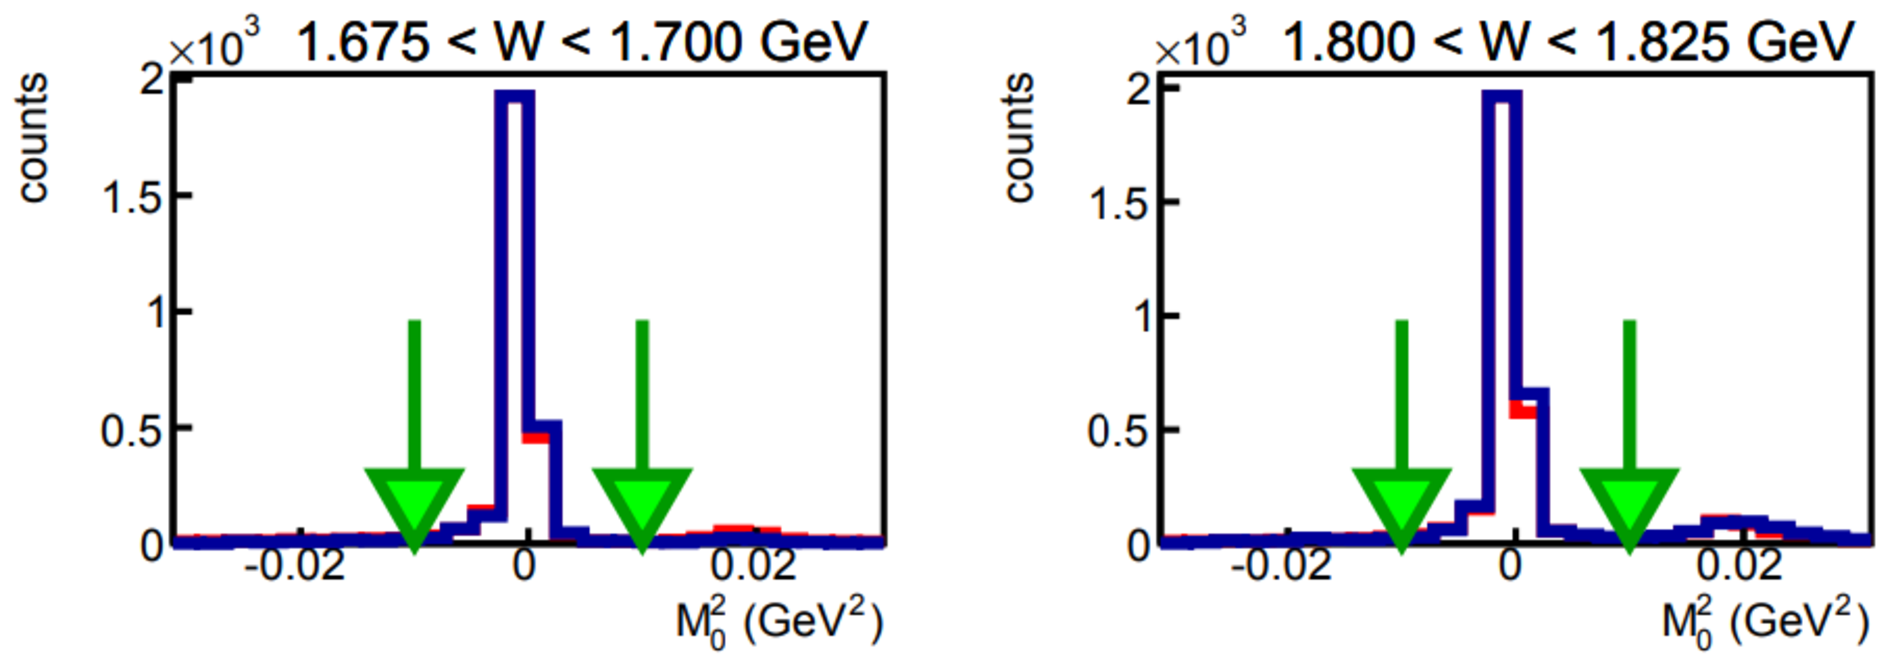
\includegraphics[width=10cm]{pictures/fed_mm0.pdf}
\end{center}
\caption{\small Distributions of the quantity $M^{2}_{X[0]}$ for the double-pion electroproduction off the free proton (taken from Ref.~\cite{fedotov_prc}). Blue histograms are for the data, red histograms are for the MC. Distributions are plotted in two 25-MeV-wide bins in $W$ specified in the plot. }  
\end{figure}

Meanwhile, if the reaction happens off a proton in the deuteron, the situation complicates. In addition to the detector resolution and radiative effects, two more factors come into play, i.e. the Fermi smearing, and FSI. Both further smear the three-pion background, with the former providing the dominant impact. As a result, the background loses its separation, adjoining the right side of the main distribution peak, which also blurs. This is seen in Fig.~2.30 of the analysis note, where the blue simulation curve shows the smearing degree for the right side the main distribution peak, and the black data curve still has a sign of peaking around $m_{\pi}^{2}$ ($\sim$0.02~GeV$^{2}$).

The three-pion background for the free proton case can be simulated as is demonstrated in FIG.~7 (here). However, the smearing of this background by the Fermi motion and FSI can hardly be simulated, especially for the latter effect. 

Note also that for the beam energy of 2~GeV, the three-pion background becomes discernible only for $W > $~1.6~GeV (though still remaining negligible) and is considered to be eliminated by the exclusivity cuts.


\item {\bf In figure 2.33 you use green vertical lines for cuts and green polynomial lines for fits to the Monte Carlo simulations. Although these are different shades of green, this is confusing. Use a different color for one of these.} \\ \\
The fit curve color was changed to cyan. 

\item {\bf In the discussion of figure 2.33 you explain how corrections are made to the yield for FSI events which are included below the green cuts. What is the systematic uncertainty in the yield arising from this process?}\\ \\
The systematic uncertainty to the cross section due to this source was estimated in the following way. The fit, shown in Fig.~2.33 (as well as the corresponding correction factor given by Eq.~(2.4.3)) turned out to be slightly dependent on the histogram binning. To account for this uncertainty, the correction factor is estimated for five different histogram bin sizes, and the arithmetic mean of these five individual values is used for the correction (for each bin in $W$). The absolute uncertainty of the resulting correction factor is estimated as a standard error of the mean (which is calculated according to Eq.~(D.4) in App.~D). The corresponding cross section uncertainty is estimated by Eq.~(D.3), where the quantity $a$ includes the number of events from the $\pi^{-}$ missing topology, while $c$ in the denominator includes the efficiency estimated for both topologies. The average value of the relative systematic uncertainty is 0.4\% among all considered $W$ and $Q^{2}$ bins.

Note that the correction is not performed (i) for $W<$~1.4875~GeV as it is not needed there and (ii) for events from the fully exclusive topology (which acquires up to $\sim$25\% of the analyzed statistics) as the procedure of the channel selection is different there. 

\item {\bf Line 934: more explanation is required of the cut 2.4.3.}\\ \\
The cut, which is shown in Fig.~2.33 by the green vertical line, is equivalent to a regular exclusivity cut, which is always performed in order to select the channel. In this study, this cut is accompanied by the corresponding correction as FSI background is not reproduced by the simulation.


This correction is very similar to the standard correction due to the cut on the photoelectrons distributions described in Sect.~2.1.1 with the correction factor given by Eq.~(2.1.13). In that case, the distributions were also subject to fitting by a smooth curve and the ratio of corresponding integrals was then obtained. 

It is also somewhat similar to the radiative correction, where the radiative correction factor is used as a multiplicative factor to the cross section value in a particular $W$ bin. 

The ending of Sect.~2.4.2 was a bit modified and rephrased in order to achieve more clarity.


\item{\bf  Table 3.1: Give range of each variable, and state whether or not the bins are of equal size. Clarify if bins are made in theta or in cos(theta) and whether they are of equal size in theta or in cos(theta). There are two sets of invariant mass bins $M_{h1h2}$ and $M_{h2h3}$. List both in the table, even if they have the same range and number of bins. Without this information the total number of bins does not relate to the product of number of bins in the five variables. Explain why there are more bins as W is increased. Is this just the case that increased cross sections allow the data to be divided into more, smaller bins, or more same-sized bins, without loss of statistical accuracy.}\\ \\
The second paragraph in Sect.~3.4 was rewritten and split into two paragraphs (page~67), which now include the information on the variable ranges, the statement that bins are of equal size for a particular $W$ subrange, and the explanation of the increasing number of bins with growing $W$. 

The specificity of the $\theta$ binning is now directly stated in the fourth paragraph of Sect.~3.4 (page~68) and at the very end of Sect.~3.5 (page~72).

The specificity of the invariant mass binning is addressed separately on the third page of Sect.~3.4 (page~69) with the invariant mass subranges given by Eq.~(3.4.1) and the bin width given by Eq.~(3.4.2). More details on the reaction phase-space are also available in App.~C. 

Both invariant masses are now listed in the Tab.~3.1.

\item {\bf Question from the annotated version on the note: (line 1182) How is the center of a multidimensional bin defined? The central value of all seven variables, or a weighted average of the events in the bin?}\\ \\
The center of a multi-dimensional bin is defined as the central value of all variables, e.g. in the 2D bin of 1.3~GeV~$<W<$~1.325~GeV and 0.5~GeV$^{2}$$<Q^{2}<$~0.55~GeV$^2$ the center is (1.3125~GeV, 0.525~GeV$^2$).



\item {\bf Figure 3.8 needs more explanation.}\\ \\
The cut in Fig.~3.8 is made to exclude the cells with unreliable efficiency from the analysis. These cells have large relative efficiency uncertainty and are clustered along the stripe-like structures. They are removed by the cut shown in the middle panel of Fig.~3.8 by the red horizontal line.

This cut is equivalent to the cut made in the study~\cite{fedotov_prc} with the only one difference, i.e. the study~\cite{fedotov_prc} used unweighted MC simulation, while this study uses weighted MC simulation. Therefore, to calculate the efficiency uncertainty $\delta \mathcal{E}$, the study~\cite{fedotov_prc} used the formula~(3.6.3) for the unweighted case, while this study has to employ the formula~(3.6.2) for the weighted case. 

Meanwhile, in the weighted simulation weights can be ignored. Then the simulation is treated as unweighted with the phase-space distributions of all kinematic variables.


Event weighing leads to some blurring of the stripe-like structures in $\delta \mathcal{E} / \mathcal{E}$ versus $\mathcal{E}$ distribution (see left panel) and in this particular case complicates the proper choice of the cut position. Therefore, the cut was applied to the distribution plotted ignoring the weights (middle panel). This also helps to observe consistency with the study~\cite{fedotov_prc}. To make sure that the procedure works as expected, the distribution for the weighted case was produced after the cut (right panel).

A separate paragraph was added into Sect.~3.6, which makes the connection between the cut in this analysis and the cut in the study~\cite{fedotov_prc}.


\item {\bf Question from the annotated version on the note: (Fig.~3.8) why are there much fewer events in (b) compared to (a) and (c). }\\ \\
The color code in Fig.~3.8 corresponds to the number of 5D cells with particular values of the efficiency and its relative uncertainty. The total number of cells (before the cut) is the same for all plots (it is 69120 for this $\Delta W \Delta Q^{2}$ bin). However, the plots have different $z$-axis maximum values, which makes this impression of ``fewer statistics". For the plot (a) the maximum was set the same as for the plot (c) to keep them in the same color spectrum (as the plot (c) is after the cut, it does not contain the horizontal stripes with cells agglomeration around zero efficiency) and to make blurred horizontal stripes in plot (a) more visible.  The plot (b) has its own $z$-axis maximum different for that of (a) and (c) as it corresponds to the unweighted case and therefore has different cell distribution.

\item {\bf Section 5.2: Can you give an argument why the off-shell effects are marginal? At present you refer to reference [41], but do not supply any physical reasons.}\\ \\
Off-shell effects, which currently are not fully explored, were not subject to the detailed investigation in this analysis as this was not among the analysis goals. The study~\cite{Ye_Tian:2017} in turn paid much attention to this issue and empirically concluded off-shell effects to have marginal impact for the deuteron target case. Therefore, to be on the safe side, we refer to the study~\cite{Ye_Tian:2017} to justify neglecting off-shell effects in this analysis.

Meanwhile, the following arguments can be considered. The binding energy of the deuterium nucleus is very small (around 2~MeV, which is just around 1~MeV per nucleon). It is the smallest among all known nuclei, it is much smaller than the nucleon mass, and it is also very small compared with the experimental beam energy, energies of the final particles and the Fermi momentum of the target nucleon as well. Therefore, such a small value of the binding energy is thought to cause a marginal effect on the cross section.

Beside this, the simulation performed with the TWOPEG-D event generator, which ignores off-shell effects, was found to describe experimental distributions well enough to conclude insignificance of these effects for this particular study.



\item {\bf Lines 1887 to 1890: You quote an average value for the systemaic error in selecting hadrons. Does this error vary appreciably with kinematic variables, e.g. at low hadron momentum? If so, it would be worth a comment describing the range of variation and the most sensitive variables.}\\ \\
The average value of this error among all $W$ and $Q^{2}$ bins is 1.6\%. However, its largest values are observed in the first two $W$ bins (with central points at 1.3125~GeV and 1.3375~GeV), with the maximum of 9.5\% achieved for the first $W$ bin at $Q^{2} = 0.675$~GeV$^{2}$. The average value of this uncertainty among the first two $W$ bins and all $Q^{2}$ bins was found to be 3.8\%.

The first two $W$ bins are located in the region very close to the reaction threshold (which is at $\sim 1.22$~GeV), which indeed corresponds to very low momenta of final hadrons. The comment on this was added to the corresponding subsection.

Note also that the total systematic uncertainty provided in the cross section plots in App.~F reflects this feature, e.g. with the average value of 7.4\% among all $W$ and $Q^{2}$ bin, the total systematic uncertainty reaches the value of 11.9\% for the first $W$ bin at $Q^{2} = 0.675$~GeV$^{2}$.

\item {\bf Figure 8.3: It would be useful to indicate the magnitude of the systematic errors in a bar at the bottom of the graphs in the second line.}\\ \\
When comparing the quasi-free cross sections with their free proton analogue, we assume that the major part of the systematic effects drops as both cross section sets were obtained under the same experimental conditions. Some effects, however, may still remain. This issue needs further investigation and will be a part of the physical interpretation of the results.



\end{enumerate}

\begin{thebibliography}{9} 



\bibitem{twopeg_d} 
 Skorodumina, {\relax Iu}. and Fedotov, G. V. and Gothe, R. W.,
\textit{``TWOPEG-D: An Extension of TWOPEG for the Case of a Moving Proton Target"}, CLAS12-NOTE-2017-014.


\bibitem{twopeg} 
 {\relax Iu} Skorodumina and G. V. Fedotov and others,
\textit{``TWOPEG: An Event Generator for Charged Double Pion Electroproduction off Proton"}, CLAS12-NOTE-2017-001.

\bibitem{Markov:2014} 
N. Markov and others,
\textit{``Single $\pi^{0}$ Electroproduction off the Proton in the Resonance region"}, CLAS-Analysis-2014-106.

\bibitem{Arjun} 
A. Trivedi and R. W. Gothe,
\textit{``Measurement of New Observables from the $p\pi^{+}\pi^{-}$ Electroproduction off the Proton"}, CLAS-Analysis-2019-102.

\bibitem{Ye_Tian:2017} 
Ye Tian and Ralf W. Gothe,
\textit{``Exclusive $\pi^{-}$ Electroproduction off the Neutron in Deuterium in the Resonance Region"}, CLAS-Analysis, under WG review.

\bibitem{fedotov_prc} 
G.~V.~Fedotov, Iu.~Skorodumina et al. [CLAS Collaboration],
\textit{``Measurements of $\gamma_{v}p \rightarrow p' \pi^{+} \pi^{-}$ cross section with the CLAS detector for 0.4 $GeV^{2}$ $< Q^2 <$ 1.0 $GeV^{2}$ and 1.3 GeV$< W <$ 1.825 GeV"}, Phys. Rev. C98 (2018) Iss. 2, 025203, arXiv:1804.05136, [see also CLAS-Note-2018-001].

\bibitem{BOS} 
\url{http://clasweb.jlab.org/bos/browsebos.php}


%\bibitem{clas_tof_paddles} 
%G. Mutcler, S. Taylor and Elton Smith,
%\textit{``CLAS TOF Scintillator Positions"}, CLAS-NOTE-1998-008.


\end{thebibliography}



 \end{document}
